\subsection{Message Broker}
A definição mais aceite de um broker de um \textit{Message Broker} é a de um software de alto nível que lida com problemas relacionados com a integração da aplicação. É tipicamente construído sobre um MOM, que providencia a base da comunicação entre as aplicações, persistência de mensagens e garantias de entrega. Modelos de \textit{Message Broker}:
\begin{itemize}
\item \textbf{Com broker} O modelo tradicional de MOM que utiliza um broker. Funciona como uma arquitectura em estrela em que todas as aplicações são ligadas através do broker e nenhuma comunicação é feita directamente. Dessa maneira as aplicações não tem necessidade de ter conhecimento da localização umas das outras, apenas o endereço do broker. A comunicação não exige que elas coexistam no espaço e no tempo além do broker ser independente das aplicações. Este mecanismo exige no entanto uma imensa troca de mensagens pela rede e todas tem de passar pelo broker podendo a levar a que se torne num \textit{bottleneck} do sistema.
\begin{figure}[H]
\centering
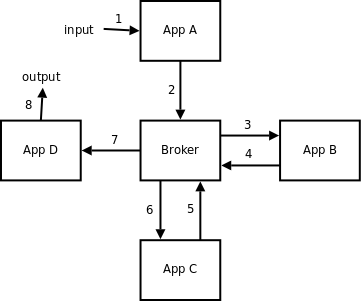
\includegraphics[width=0.65\textwidth]{broker1.png}
\caption{\textit{Arquitectura com Broker}}
\label{fig:broker}
\end{figure}
\item \textbf{Sem broker}\\
A imagem mostra um cenário em que não existe broker.
\begin{figure}[H]
\centering
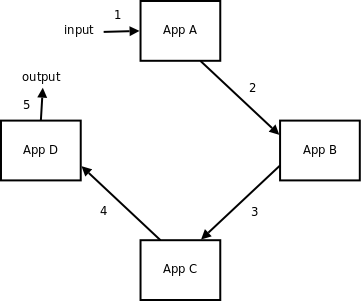
\includegraphics[width=0.65\textwidth]{nobroker.png}
\caption{\textit{Arquitectura sem Broker}}
\label{fig:nobroker}
\end{figure}
O número de mensagens decresce e não existe nenhum tipo de limitação do género \textit{bottleneck} como no exemplo anterior. Este tipo de arquitectura é ideal para sistemas com exigências de baixa latência de comunicação e com alta taxa de transacções. Cada aplicação apenas tem de se conectar com a aplicação ou aplicações com que faz a comunicação, tendo de saber o endereço de cada uma delas. Apesar de ser aceitável neste exemplo simples,  No  mundo real não tem aplicação porque nesses casos existem centenas de milhares de aplicações ligadas. Fazer a gestão dessas ligações todas seria um trabalho muito custoso.\\
\item \textbf{Broker como serviço de Directorias} \\
A funcionalidade do broker pode ser dividida em duas partes separadas. Primeiro, o broker como um repositório de aplicações a correr na rede. Sabe que a aplicação X corre num host Y e que as mensages para X devem ser mandadas para Y. Age como um serviço de directorias. Segundo, o broker faz a troca de mensagens ele mesmo.\\
Para resolver problemas de gestão, a tarefa de troca de mensagens pode ser feita pelas aplicações. Uma aplicação X pode registar ao broker que corre no host Y. A aplicação Z quer envias uma mensagem para a aplicação X vai "questionar" o broker sobre a localização de X. Assim que a resposta de que X está em Y chegar a Z, Z pode criar uma conecção directa para Y e enviar a mensagem por ele mesmo sem incomodar o broker. A imagem em baixo ilustra a arquitectura:\\
\begin{figure}[H]
\centering
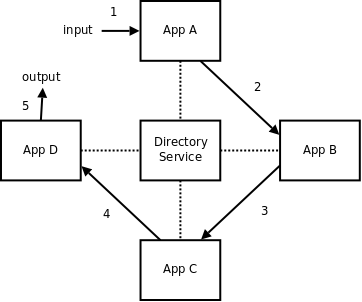
\includegraphics[width=0.65\textwidth]{dsbroker.png}
\caption{\textit{Broker como Serviço de directorias}}
\label{fig:dsbroker}
\end{figure}
Dessa maneira é possível obter uma maior performance e tornar o sistema mais fácil de gerir ao mesmo tempo.
\item \textbf{Broker Distribuído}\\
Para atingir o tipo de comportamento suposto para um \textit{Message Broker} é apenas necessário um broker no meio, mas não é possível evitar o problema do broker como \textit{bottleneck}. Uma arquitectura distribuída evita esse problema.\\
\begin{figure}[H]
\centering
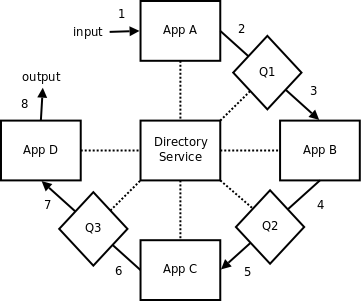
\includegraphics[width=0.65\textwidth]{dbroker.png}
\caption{\textit{Broker distribuído}}
\label{fig:distributedbroker}
\end{figure}
Como podemos ver pela imagem, cada fila de mensagen é implementada como aplicação separada. Pode correr no mesmo host que aplicação a que esta ligado ou pode correr num host completamente diferente. Muitas filas podem correr num simples host, o host pode ser dedicado exclusivamente a ter apenas uma fila. A fila é registada com o broker e assim é acessível a todas as aplicações na rede. A fila é uma peça de software bastante simples que recebe mensagens dos emissores e distribui pelos receptores. A change de falhar é bastante mais baixa que aplicações reais cheias de complexidade de negócio.
\end{itemize}


